\section{Risultati}
Per confrontare gli attacchi è stato eseguito $run\_benchmark$ sulla suite di percorsi $regular$.
Questa suite è composta da 4 mappe con determinate caratteristiche:\begin{itemize}
    \item NoCrashTown01-v3\begin{itemize}
        \item numero di veicoli:20
        \item numero di pedoni:50
    \end{itemize}
    \item NoCrashTown02-v3 \begin{itemize}
        \item numero di veicoli:15
        \item numero di pedoni:50
    \end{itemize}
    \item NoCrashTown01-v4 \begin{itemize}
        \item numero di veicoli:20
        \item numero di pedoni:50
    \end{itemize}
    \item NoCrashTown02-v4 \begin{itemize}
        \item numero di veicoli:15
        \item numero di pedoni:50
    \end{itemize}
\end{itemize}
Ciascuna mappa prevede l'esecuzione di tre percorsi, ognuno con  condizioni ambientali diverse. 
La valutazione degli attacchi si è svolta in due fasi:\begin{itemize}
    \item nella prima, i percorsi sono stati seguiti da un agente "puro", senza nessun attacco iniettato
    \item nella seconda fase, si eseguono le stesse run della prima fase, ma ogni volta con un diverso attacco iniettato.
\end{itemize}
I risultati prodotti dall'iniezione di ciascun attacco sono stati confrontati con quelli prodotti dalla run pura, in modo da valutarne l'efficacia.
Il confronto  è stato fatto sia in termini di percorsi portati a termine, sia andando ad analizzare e commentare i video prodotti.
\subsection{Golden Run}
\begin{table}[h]
    \begin{tabular}{|c|c|c|}
        \hline
        Mappa                   & Run completate & Percentuale di completamento\\
        \hline
        NoCrashTown01-v3        & 3/3            & 100\% \\
        NoCrashTown01-v4        & 3/3            & 100\% \\
        NoCrashTown02-v3        & 3/3            & 100\% \\
        NoCrashTown02-v4        & 3/3            & 100\%  \\
        Totale                  & 12/12          & 100\% \\
        \hline
    \end{tabular}
    \caption{risultati golden run}
Nella golden run tutti i percorsi vengono completati con successo. La traiettoria del veicolo è stabile e un solo semaforo rosso in totale è stato ignorato.
\end{table}
\begin{figure}[h!]
    \centering
    \parbox{6cm}{
    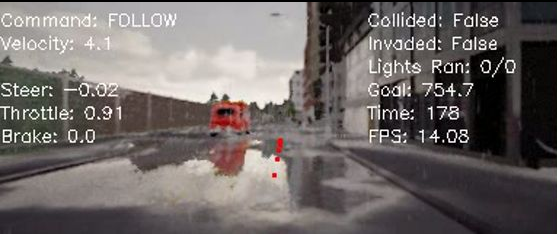
\includegraphics[width=6cm]{GOLD1.png}
    \label{fig:gold1}}
    \qquad
    \begin{minipage}{6cm}
    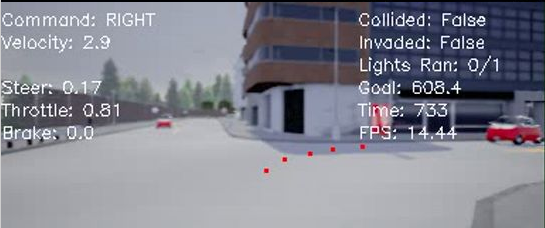
\includegraphics[width=6cm]{GOLD2.png}
    \label{fig:gold2}
    \end{minipage}
    \label{fig:goldrun}
    \end{figure}
\newpage
\subsection{Iniezione di HopSkipJump (HSJ)}
\begin{table}[h!]
    \begin{tabular}{|c|c|c|}
        \hline
        Mappa                   & Run completate & Percentuale di completamento\\
        \hline
        NoCrashTown01-v3        & 3/3            & 100\% \\
        NoCrashTown01-v4        & 2/3            & 66\% \\
        NoCrashTown02-v3        & 1/3            & 33\% \\
        NoCrashTown02-v4        & 0/3            & 0\%  \\
        TOTALE                  & 6/12           & 50\% \\
        \hline
    \end{tabular}
    \caption{risultati run HopSkipJump}
    \label{tab:hsj}
\end{table}
 Fallimento parziale del veicolo. Dall'analisi video si nota una guida molto più instabile ma che continua all'incirca
a seguire il percorso prestabilito. L'instabilità è particolarmente evidente negli waypoints prodotti, che cambiano continuamente posizione anche nei rettilinei. A causa dei problemi elencati
si nota un aumento dei semafori ignorati, delle uscite fuori strada e delle collisioni con altri oggetti.
\begin{figure}[h]
    \centering
    \parbox{6cm}{
    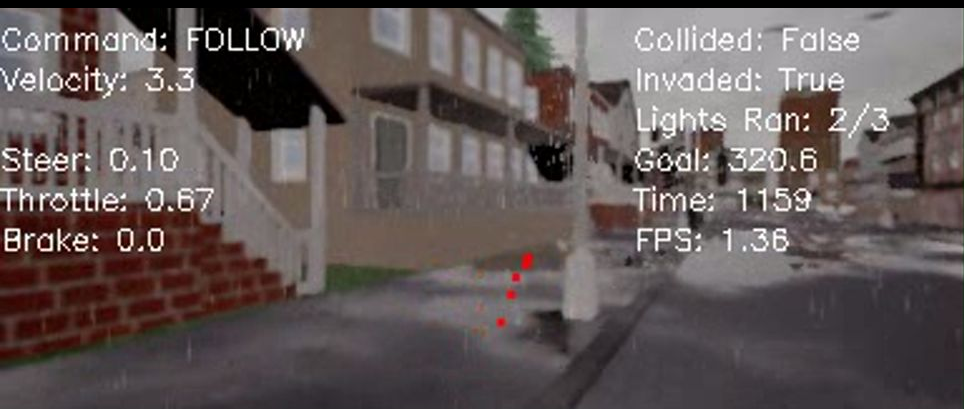
\includegraphics[width=6cm]{hoprun.png}
    \label{fig:hop1}}
    \qquad
    \begin{minipage}{6cm}
    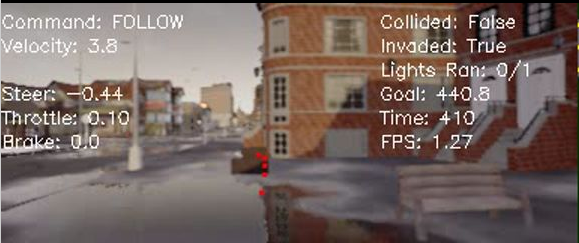
\includegraphics[width=6cm]{HOP2.png}
    \label{fig:hop2}
    \end{minipage}
    \label{fig:hoprun}
    \end{figure}
\subsection{Iniezione di Spatial Transformation}
\begin{table}[h!]
    \begin{tabular}{|c|c|c|}
        \hline
        Mappa                   & Run completate & Percentuale di completamento\\
        \hline
        NoCrashTown01-v3        & 2/3            & 66\% \\
        NoCrashTown01-v4        & 3/3            & 100\% \\
        NoCrashTown02-v3        & 1/3            & 33\% \\
        NoCrashTown02-v4        & 1/3            & 33\%  \\
        TOTALE                  & 7/12           & 0\% \\
        \hline
    \end{tabular}
    \caption{risultati run Spatial Transformation (STA)}
    \label{tab:sta}
\end{table}
Moderato fallimento del veicolo. La traiettoria continua a essere seguita in modo abbastanza fedele ma la guida risulta più instabile.
La maggior parte dei percorsi è fallito per il tempo scaduto, ma sono comparse anche delle collisioni. Nessun semaforo ignorato.
\begin{figure}[h]
    \centering
    \parbox{6cm}{
    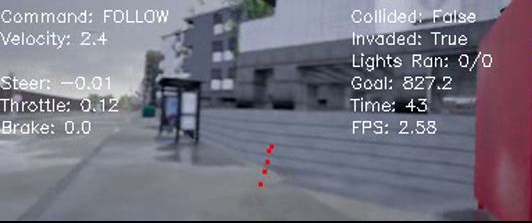
\includegraphics[width=6cm]{STA1.png}
    \label{fig:sta1}}
    \qquad
    \begin{minipage}{6cm}
    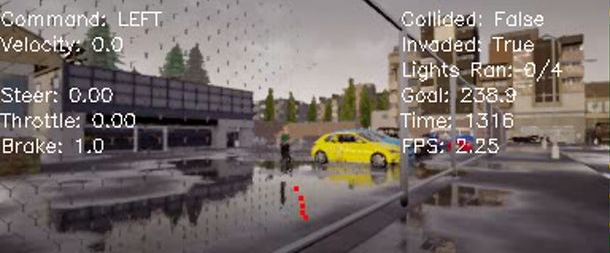
\includegraphics[width=6cm]{STA2.png}
    \label{fig:sta2}
    \end{minipage}
    \label{fig:starun}
    \end{figure}
\subsection{Iniezione di Basic Iterative Method(BIM)}
\begin{table}[h!]
    \begin{tabular}{|c|c|c|}
        \hline
        Mappa                   & Run completate & Percentuale di completamento\\
        \hline
        NoCrashTown01-v3        & 0/3            & 0\% \\
        NoCrashTown01-v4        & 0/3            & 0\% \\
        NoCrashTown02-v3        & 0/3            & 0\% \\
        NoCrashTown02-v4        & 0/3            & 0\%  \\
        TOTALE                  & 0/12           & 0\% \\
        \hline
    \end{tabular}
    \caption{risultati run Basic Iterative Method}
    \label{tab:bim}
\end{table}
Avviene un fallimento totale del veicolo. In nessuno dei percorsi la macchina inizia a seguire il tragitto, ma invece inizia a sterzare verso destra fino ad uscire di strada
e  urtare oggetti della mappa.
\begin{figure}[h]
    \centering
    \parbox{6cm}{
    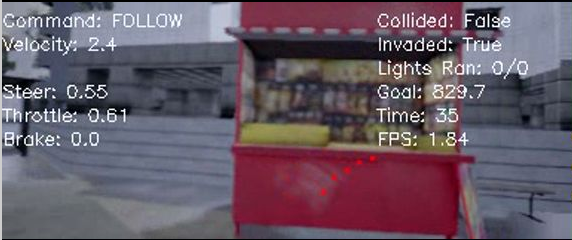
\includegraphics[width=6cm]{BIM1.png}
    \label{fig:bim1}}
    \qquad
    \begin{minipage}{6cm}
    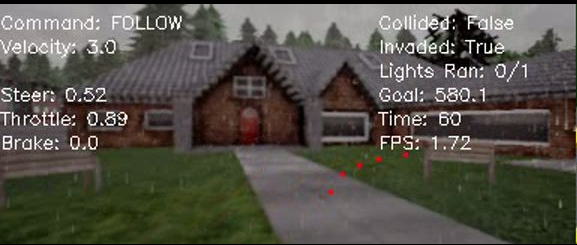
\includegraphics[width=6cm]{BIM2.png}
    \label{fig:bim2}
    \end{minipage}
    \label{fig:bimrun}
    \end{figure}
\subsection{Iniezione di NewtonFool (NF)}
\begin{table}[h!]
    \begin{tabular}{|c|c|c|}
        \hline
        Mappa                   & Run completate & Percentuale di completamento\\
        \hline
        NoCrashTown01-v3        & 1/3            & 33\% \\
        NoCrashTown01-v4        & 2/3            & 66\% \\
        NoCrashTown02-v3        & 0/3            & 0\% \\
        NoCrashTown02-v4        & 0/3            & 0\%  \\
        TOTALE                  & 3/12           & 25\% \\
        \hline
    \end{tabular}
    \caption{risultati run NewtonFool}
    \label{tab:nf}
\end{table}
Fallimento grave del veicolo. Il tragitto viene seguito ma con una traiettoria molto instabile. Aumento rilevante dei semafori rossi ignorati e delle collisioni.
\begin{figure}[h]
    \centering
    \parbox{6cm}{
    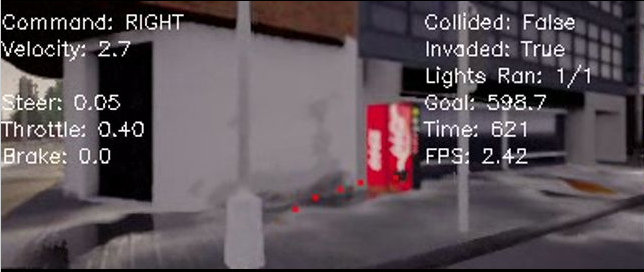
\includegraphics[width=6cm]{FOOL1.png}
    \label{fig:fool1}}
    \qquad
    \begin{minipage}{6cm}
    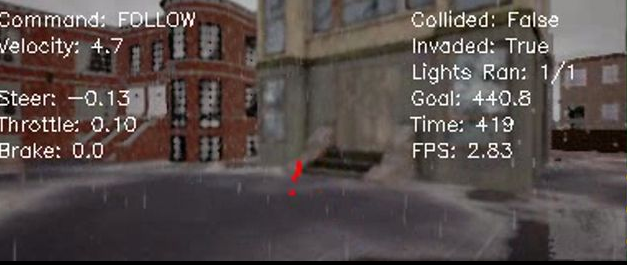
\includegraphics[width=6cm]{FOOL2.png}
    \label{fig:fool2}
    \end{minipage}
    \label{fig:foolrun}
    \end{figure}
\subsection{Sintesi risultati}
I risultati riassunti nella Tabella \ref{tab:ria} ci dimostrano la vulnerabilità del modello considerato agli adversarial attacks. In tutti i casi l'affidabilità del veicolo si è ridotta.
L'attacco che ha causato problemi più gravi è sicuramente Basic Iterative Method. Mentre nelle altre run la traiettoria prestabilita continua ad essere quantomeno seguita, in questo
caso la macchina cambia completamente comportamento, diventando inutilizzabile.
\begin{table}[h]
    \begin{tabular}{|p{1.5cm}|p{2.5cm}|p{2cm}|p{1.5cm}|c|c|}
        \hline
        Attacco        &   Run completate     &   stabilità     &  semafori ignorati        & collisioni & timeout\\
        \hline
        Nessuno        &  12/12               &   ottima        &  1                        & 0          & 0 \\
        HSJ            &  6/12                &   bassa         &  9                        & 6          & 0 \\
        STA            &  7/12                &   buona         &  0                        & 4          & 1 \\
        BIM            &  0/12                &   nulla         &  N/D                      & 12         & 0\\
        NF             &  3/12                &   bassa         &   13                      & 9          & 0 \\
        \hline
    \end{tabular}
    \caption{tabella riassuntiva}
    \label{tab:ria}
\end{table}